\chapter{Analysis}

\section{Revenue Analysis}
\begin{table}[htbp]
    \centering
    \small
    \caption{Value added by the battery over the no-battery household, before aging,
    by the spot price of the interval in which it was earned (\$).}
    \label{tab:mpc:bands}
    \begin{tabular}{@{}lrrrrrr@{}}
        \toprule
        $R_n$ (\$/MWh) & Intervals & Perfect & \shortstack{Perfect\\price} & Naive & AEMO & LSTM \\
        \midrule
        $< 0$       & 1411 & 2.35   & $-0.49$ & 0.15   & $-0.25$ & $-0.07$ \\
        0 -- 50     & 1211 & $-1.20$ & $-3.14$ & $-3.04$ & $-3.02$ & $-3.18$ \\
        50 -- 100   & 3928 & 2.02   & 1.40   & 1.44   & 1.37   & 0.79 \\
        100 -- 300  & 2338 & 23.89  & 20.69  & 17.22  & 18.65  & 19.87 \\
        300 -- 1000 & 30   & 6.57   & 5.65   & 5.71   & 4.24   & 5.66 \\
        $> 1000$    & 10   & 101.53 & 101.53 & 101.53 & 100.56 & 101.53 \\
        \midrule
        Total       & 8928 & 135.16 & 125.64 & 123.01 & 121.55 & 124.60 \\
        \bottomrule
    \end{tabular}
\end{table}

\paragraph{Three quarters of the value is earned in ten intervals, and every controller captures it.}
Table~\ref{tab:mpc:bands} separates the value added by price band. Of the \$135.16 added
under perfect foresight, \$101.53 is earned in the 50 minutes during which the price
exceeded \$1000/MWh. All five controllers discharge at the full 11.04~kW in those
intervals, with the single exception of the AEMO-driven controller in the
\$1052/MWh interval on 14 January, at a cost of \$0.97. This occurs because the price of
the current interval is observed before dispatch, and because each controller happened
to be holding charge when each spike arrived. None of the forecasters predicted these
spikes, and none needed to. The differences between forecasters arise instead in
ordinary arbitrage: in the \$100 to \$300/MWh band, where perfect foresight earns
\$23.89 against \$17.22 to \$20.69, and at negative prices, where it earns \$2.35
against approximately zero.

\section{Sensitivity Analysis}
\subsection{Price}

\subsection{Net-Demand}
\subsubsection{Sensitivity to forecast error}
\label{sec:results:mpc:noise}

The real forecasters give three points, each with a different kind of error. To measure
how dispatch value depends on the \emph{size} of the error alone, the MPC study was
repeated with perfect foresight corrupted by synthetic error of controlled magnitude,
applied to one input at a time while the other was kept perfect. A forecast issued at
interval $t$ for lead $h = 0, \dots, 287$ is
\begin{equation}
    \hat{x}_{t+h} = x_{t+h} + \sigma_{\max} \sqrt{\tfrac{h+1}{288}}\, e_h,
    \qquad e_h = \rho\, e_{h-1} + \sqrt{1-\rho^2}\, \varepsilon_h, \quad \varepsilon_h \sim \mathcal{N}(0,1),
    \label{eq:noise}
\end{equation}
with $e_0 \sim \mathcal{N}(0,1)$ and $\rho = 0.95$ per five-minute step, so that errors
persist for about 1.5~hours rather than alternating between intervals, and grow with lead
time to $\sigma_{\max}$ at 24~hours. For price, $x = \sinh^{-1}(R/100)$, the transform
used by the LSTM, and the forecast is returned as $100 \sinh(\hat{x})$; the error is
therefore approximately additive near zero and proportional during spikes. For net
local power, $x = G - A$ in kW. A new error path is drawn at every re-plan, and the
current-interval price remains the actual price. Independent errors in each interval
were rejected because the MILP would trade on the spurious five-minute spreads they
create. One realisation is used per level; each run averages 8928 independent draws.

\begin{table}[htbp]
    \centering
    \small
    \caption{Dispatch value under synthetic forecast error, household scenario, $J=4$,
    January 2025. Each run perturbs one input; the other is perfect. Value lost is
    measured against perfect foresight on the same loop.}
    \label{tab:mpc:noise}
    \begin{tabular}{@{}llrrrrrr@{}}
        \toprule
        Input & $\sigma_{\max}$ & MAE & \shortstack{Profit\\at meter (\$)} &
        \shortstack{Rainflow\\deg.\ (\$)} & \shortstack{Net\\profit (\$)} &
        \shortstack{Value\\lost (\$)} & EFC \\
        \midrule
        None      & --      & --           & 43.31 & 15.07 & 28.24 & --    & 9.3 \\
        \midrule
        Price     & 0.25    & 19.8 \$/MWh  & 43.68 & 15.58 & 28.10 & 0.14  & 9.6 \\
                  & 0.5     & 41.1 \$/MWh  & 44.67 & 16.92 & 27.75 & 0.49  & 10.4 \\
                  & 1       & 95.9 \$/MWh  & 45.16 & 20.77 & 24.38 & 3.86  & 12.7 \\
                  & 2       & 388.3 \$/MWh & 34.29 & 33.80 & 0.50  & 27.74 & 23.1 \\
        \midrule
        Net local & 0.5 kW  & 0.27 kW      & 43.11 & 15.20 & 27.92 & 0.32  & 9.4 \\
                  & 1 kW    & 0.53 kW      & 42.88 & 15.23 & 27.64 & 0.60  & 9.5 \\
                  & 2 kW    & 1.06 kW      & 42.37 & 15.33 & 27.04 & 1.20  & 9.6 \\
                  & 3 kW    & 1.60 kW      & 42.01 & 15.42 & 26.58 & 1.66  & 9.7 \\
        \bottomrule
    \end{tabular}
\end{table}

\begin{figure}[htbp]
    \centering
    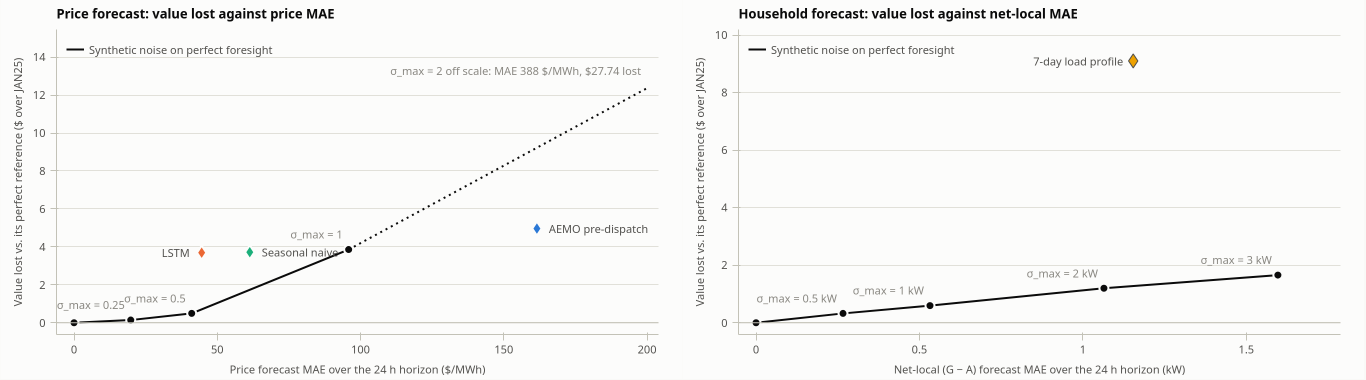
\includegraphics[width=\textwidth]{images/forecast_noise_sensitivity.png}
    \caption{Value lost against forecast MAE. The curve is synthetic error on perfect
    foresight (Table~\ref{tab:mpc:noise}); the points are the forecasters of
    Table~\ref{tab:mpc:headline}, each measured against the reference that isolates its
    input: the price forecasters against the perfect-price case, the seven-day household
    profile against perfect foresight.}
    \label{fig:mpc:noise}
\end{figure}

% STALE (2026-09-30): Table mpc:noise is on the corrected (interval-end) meter data. The
% real-forecaster points in Fig. mpc:noise and the comparisons below use
% Table mpc:headline, which is still from the old join; re-run forecast_trading.py.
Perfect foresight on the corrected data nets \$28.24, which again matches the 48-hour
rolling solve of Table~\ref{tab:milp:household}.

\paragraph{Unbiased error is cheap until it is large.}
Price error with an MAE of \$41/MWh, comparable to the LSTM, costs \$0.49, and an MAE
of \$96/MWh costs \$3.86. Only at an MAE of \$388/MWh is the value almost eliminated.
Household error costs about \$1 per kW of MAE over the range tested.

\paragraph{Price error costs through cycling, not through worse trades.}
Up to $\sigma_{\max} = 1$ the profit at the meter \emph{rises}, from \$43.31 to
\$45.16. The controller acts on spreads that the error has widened, cycling 12.7
equivalent full cycles instead of 9.3, and the additional rainflow degradation of
\$5.70 exceeds the additional revenue. The degradation cost in the objective restrains
this, but it cannot distinguish a real spread from a forecast one.

\paragraph{The real forecasters lose far more than their MAE predicts.}
Figure~\ref{fig:mpc:noise} places the real forecasters on the synthetic curve. The
seven-day household profile has an MAE of 1.15~kW, at which unbiased error would cost
about \$1.28; it costs \$9.10. The LSTM and seasonal-naive price forecasts, at \$45 and
\$61/MWh, would cost about \$0.71 and \$1.74; each costs about \$3.70. The loss is
therefore driven by the structure of the error rather than its size. The synthetic error
is unbiased and independent of the data, so it averages out over the month. A real
forecast is wrong in a way that depends on the day, for example a seven-day profile on a
cloudy day or a price forecast that flattens the daily shape, and such errors move the
whole schedule in the same direction. Which features of the error are responsible has
not been isolated here. AEMO
pre-dispatch sits below the curve, because most of its MAE comes from forecast spikes
that did not occur, and these are corrected by the observed current-interval price
before they affect dispatch. MAE is therefore a poor guide to the dispatch value of a
forecast in either direction, consistent with the loose relation between accuracy and
value found above.


\section{Forecaster Analysis}

\section{Constrained Grid Connection}
\paragraph{The result depends on an unconstrained grid connection.}
No export limit is enforced in the runs above, and during the price spikes the household
exports up to 14~kW, the full 11.04~kW of the battery in addition to the solar
surplus. Table~\ref{tab:milp:export} repeats the household $J = 4$ run with the grid
export limited to 10~kW and to 5~kW, the latter being a common limit for a single-phase
connection. Solar curtailment is not modelled, so under a limit the battery must also
keep headroom for any surplus above it. A 5~kW limit removes 40\% of the value added by
the battery, almost all of it from the spike intervals, and the net profit of the
household becomes a net cost. The value outside the spike intervals is nearly
unaffected.

\begin{table}[htbp]
    \centering
    \small
    \caption{Perfect-foresight MILP, household scenario, $J=4$, under a grid export limit,
    January 2025 (\$). Value added is measured against the no-battery household and is
    before aging.}
    \label{tab:milp:export}
    \begin{tabular}{@{}lrrrrr@{}}
        \toprule
        Export limit & \shortstack{Profit\\at meter} & \shortstack{Rainflow\\deg.} &
        \shortstack{Net\\profit} & \shortstack{Value\\added} &
        \shortstack{of which\\$R_n > 1000$} \\
        \midrule
        None  & 43.31     & 15.07 & 28.25     & 135.11 & 101.55 \\
        10~kW & 35.16     & 15.01 & 20.14     & 126.95 & 93.65 \\
        5~kW  & $-10.63$  & 14.37 & $-25.00$  & 81.17  & 49.00 \\
        \bottomrule
    \end{tabular}
\end{table}

\paragraph{No-battery reference.}
On spot settlement the household alone pays \$102.04 for imports and receives \$10.24 for
exports, a net position of $-$\$91.80 for the month. Household results below are the
net position of the whole household, so the value added by the battery is the reported
result minus $-$\$91.80.

\section{Retail self-consumption}
\subsection{Comparison of operating models}
\label{sec:results:comparison}

Table~\ref{tab:comparison} expresses each result as the value added by the battery over
the same household with no battery under the same pricing arrangement.

\begin{table}[htbp]
    \centering
    \small
    \caption{Value added by the battery over the no-battery household, January 2025 (\$).}
    \label{tab:comparison}
    \begin{tabular}{@{}lrrr@{}}
        \toprule
        Operating model & \shortstack{Gross value\\added} & \shortstack{Rainflow\\deg.} &
        \shortstack{Net value\\added} \\
        \midrule
        Spot, perfect foresight, $J=4$               & 135.11 & 15.07  & 120.04 \\
        Spot, LSTM-driven MPC                        & 124.60 & 17.35  & 107.25 \\
        Spot, seasonal-naive MPC                     & 123.01 & 15.79  & 107.23 \\
        Spot, perfect foresight, 5~kW export limit   & 81.17  & 14.37  & 66.80 \\
        Spot, degradation ignored                    & 186.84 & 194.62 & $-7.78$ \\
        \midrule
        Retail time of use, optimised, perfect foresight & 61.61 & 25.47 & 36.14 \\
        Retail single rate, optimised, perfect foresight & 30.20 & 12.38 & 17.82 \\
        Retail time of use, self-consumption rule    & 71.21  & 63.36  & 7.85 \\
        Retail single rate, self-consumption rule    & 55.94  & 63.36  & $-7.42$ \\
        \bottomrule
    \end{tabular}
\end{table}

The rows must be compared like for like. The perfect-foresight spot result and the
optimised retail results use the same optimiser, the same aging cost and the same
foresight, and differ only in the prices: \$120.04 on spot prices against \$36.14 and
\$17.82 on the retail plans. The forecast-driven spot results and the self-consumption
rule are both realisable, the rule needing no forecast at all: about \$107 on spot
prices against \$7.85 and $-$\$7.42. Comparing a degradation-aware spot controller with
the degradation-blind rule would attribute to the tariff a difference in battery wear
that belongs to the controller.

On either comparison spot exposure is worth substantially more in this month, and
approximately \$100 of the difference is earned in the ten spike intervals. With those
intervals excluded the ranking reverses. Perfect foresight on spot prices adds \$33.56
before aging and \$18.49 after it, level with the optimised single-rate result and half
of the optimised time-of-use result. The LSTM-driven controller adds \$23.07 before
aging and \$5.72 after it, which is within the range of the self-consumption rule. The
case for spot exposure in this month therefore rests entirely on the price spikes, and
on a grid connection that allows the battery to export at full power during them: under
a 5~kW export limit the perfect-foresight spot result falls to \$66.80.

% -----------------------------------------------------------------------------
\subsection{Limitations}
\label{sec:results:limitations}

The results cover one month, one household and one region. January has the highest solar
generation of the year and in 2025 contained one day on which the price reached the
market price cap and a second on which it exceeded \$15\,000/MWh. The spot results should not be annualised, since three quarters of the
value was earned in ten intervals.

The degradation inputs are generic. The replacement cost of \$10\,800 is an installed
price, which is an upper estimate of the cost of replacing the cells, and the stress
function is that of NMC cells, which overstates the aging of a battery built from
lithium iron phosphate cells. The sign of
the single-rate result of the self-consumption rule and the size of every net figure
depend on both. The
gross figures do not, although the schedules produced by the degradation-aware MILP do.

Spot exposure is modelled without a retailer. No subscription fee, retail margin or
daily supply charge is applied on the spot side, whereas the retail bills include a
supply charge of \$46 to \$49. The spot side also omits GST, environmental scheme
costs, market fees and distribution loss factors: the retail rates include GST, while
the spot price and the network tariff are used as published.
% TODO: confirm that the Ausgrid EA010 rate of 10.8007 c/kWh excludes GST.
The spot import price is therefore understated by at least 10\%, which is visible in the
no-battery energy cost of \$91 on spot prices against \$122 on the single-rate plan
before the supply charge. The value added by the battery is less sensitive to this than
the bills are, since each is measured against its own no-battery case, but every
kilowatt-hour the battery imports or displaces is affected. The spot side also uses a
flat network tariff, whereas the time-of-use retail plan is built on a time-of-use
network tariff.

The price of the current interval is taken as known for the whole interval. In practice
it is published at about the start of the interval, and a delay of 30 to 60~seconds in
receiving and acting on it would forgo 10\% to 20\% of the energy discharged in a spike
interval.

Apart from Table~\ref{tab:milp:export}, no grid import or export limit is enforced. The
household solar is treated as a separate flow that does not share the 11.04~kW inverter
of the battery, solar curtailment is not modelled, efficiencies are fixed, and calendar
aging is not modelled. The state machine operates a 20~kWh lossless battery, so its
result is a qualitative comparison only.

\section{Observable State Space}
\label{sec:analysis:observable_state}
Describe the impacts that changing the observable state space for the system demand had and why